\section{Проектирование архитектуры}
\label{sec:architecture-design}

При проектировании архитектуры системы применялись принципы чистой архитектуры~\cite{martin2018}, паттерны проектирования распределённых систем~\cite{kleppmann2017,gamma1994} и нотации визуального моделирования~\cite{booch2006}. Репозиторный слой реализован в соответствии с паттерном Repository, описанным в~\cite{fowler2002}.

\subsection{Диаграмма контекста системы}

На рисунке~\ref{fig:c4-context} представлена диаграмма контекста системы Guide Helper, показывающая систему в окружении внешних пользователей и сервисов.

Система взаимодействует с четырьмя внешними сервисами:
\begin{itemize}
  \item OpenStreetMap / Yandex Maps~--- предоставляет картографические тайлы для отображения интерактивной карты;
  \item Open-Meteo~--- предоставляет данные о высоте рельефа и прогноз погоды;
  \item Nominatim~--- сервис геокодирования для поиска местоположений по названию;
  \item ИИ-провайдеры и OpenAI-совместимые шлюзы~--- используются для
    ИИ-ассистента и генерации описаний маршрутов по фотографиям.
\end{itemize}

\begin{figure}[H]
  \centering
  
\includegraphics[width=0.95\textwidth]{images/c4-context.png}
  \caption{Диаграмма контекста системы}
  \label{fig:c4-context}
\end{figure}

\subsection{Диаграмма контейнеров}

На рисунке~\ref{fig:c4-container} представлена диаграмма контейнеров, детализирующая внутреннюю структуру системы.

Система состоит из следующих контейнеров:
\begin{itemize}
  \item клиентская часть~--- одностраничное приложение на React~19 с TypeScript, интерактивные карты на Leaflet, прогрессивное веб-приложение и настольная оболочка Tauri, поддержка тем оформления;
  \item сервис аутентификации~--- микросервис на Rust (Axum), JWT-токены, Argon2, ролевая модель (пользователь/модератор/администратор);
  \item сервис маршрутов~--- микросервис управления маршрутами на Rust (Axum), REST API, WebSocket, потоковая передача событий (SSE), ИИ-ассистент с вызовом инструментов, генерация описаний маршрутов, уведомления, категории, закладки;
  \item обработчик фотографий~--- микросервис на Rust, потребитель очереди NATS; выполняет асинхронную обработку изображений и обновляет их статус;
  \item сервис кэширования~--- микросервис кэширования тайлов на Go (Gin), Redis;
  \item сервис тайлов~--- микросервис проксирования тайлов карт на Go (Gin);
  \item PostgreSQL~--- СУБД (две базы: auth\_db и routes\_db; routes\_db содержит таблицы маршрутов, категорий, комментариев, закладок, уведомлений и сообщений чата);
  \item Redis~--- кэш тайлов карт;
  \item NATS JetStream~--- брокер сообщений для асинхронной обработки фотографий;
  \item MinIO~--- S3-совместимое объектное хранилище для фотографий.
\end{itemize}

\begin{figure}[H]
  \centering
  
\includegraphics[width=0.95\textwidth]{images/c4-container.png}
  \caption{Диаграмма контейнеров системы}
  \label{fig:c4-container}
\end{figure}

\subsection{Диаграмма последовательности обработки фотографий}

На рисунке~\ref{fig:sequence-photo} представлена диаграмма последовательности, описывающая процесс асинхронной обработки фотографий~--- одного из ключевых сценариев работы системы.

Процесс состоит из следующих шагов:
\begin{enumerate}
  \item Пользователь загружает фотографию через веб-интерфейс.
  \item Фронтенд извлекает GPS-координаты из EXIF-метаданных фотографии.
  \item Фронтенд отправляет фотографию и координаты на сервис маршрутов.
  \item Сервис маршрутов сохраняет точку маршрута с фотографией в статусе <<ожидает обработки>> в PostgreSQL.
  \item Сервис маршрутов публикует сообщение в NATS JetStream с метаданными для обработки.
  \item Обработчик фотографий получает сообщение из очереди NATS.
  \item Обработчик фотографий выполняет обработку: сжатие, масштабирование, генерацию миниатюры.
  \item Обработчик фотографий загружает обработанные файлы в MinIO.
  \item Обработчик фотографий обновляет запись в PostgreSQL: адреса файлов и статус <<выполнено>>.
  \item Сервис маршрутов отправляет уведомление через WebSocket в клиентское приложение.
  \item Фронтенд обновляет отображение фотографии на карте.
\end{enumerate}

\begin{figure}[H]
  \centering
  
\includegraphics[width=0.95\textwidth]{images/sequence-photo.png}
  \caption{Диаграмма последовательности обработки фотографий}
  \label{fig:sequence-photo}
\end{figure}

\subsection{Проектирование базы данных}

Система использует две отдельные базы данных PostgreSQL для обеспечения изоляции сервисов.

База данных auth\_db содержит таблицу \texttt{users} для хранения учётных данных пользователей: идентификатор (UUID), адрес электронной почты, хеш пароля (Argon2), имя, адрес аватара, временные метки создания и обновления, поддержка мягкого удаления.

База данных routes\_db содержит следующие таблицы:
\begin{itemize}
  \item routes~--- маршруты (UUID, идентификатор пользователя, название, точки в JSONB, описание, сезонность, токен публикации, поля версионирования);
  \item categories~--- категории маршрутов (UUID, название);
  \item route\_categories~--- связь маршрутов и категорий (отношение многие-ко-многим);
  \item comments~--- комментарии к маршрутам;
  \item route\_likes~--- отметки «нравится» (пара идентификаторов маршрута и пользователя);
  \item route\_ratings~--- рейтинги маршрутов (1--5 баллов, уникальная пара идентификаторов);
  \item route\_bookmarks~--- закладки (избранные маршруты пользователя);
  \item notifications~--- уведомления пользователей о комментариях, отметках и рейтингах;
  \item settings~--- прикладные настройки сервиса маршрутов;
  \item chat\_messages~--- сообщения диалогов (роль: пользователь/ассистент, \texttt{conversation\_id}, контент, действия в JSONB).
\end{itemize}

Точки маршрута хранятся в поле \texttt{points} типа JSONB в таблице \texttt{routes}. Каждая точка содержит: идентификатор, координаты (широта, долгота) и опциональные данные фотографии (адрес оригинала, адрес миниатюры, статус).

ER-диаграмма базы данных представлена на рисунке~\ref{fig:er-diagram}.

\begin{figure}[H]
  \centering
  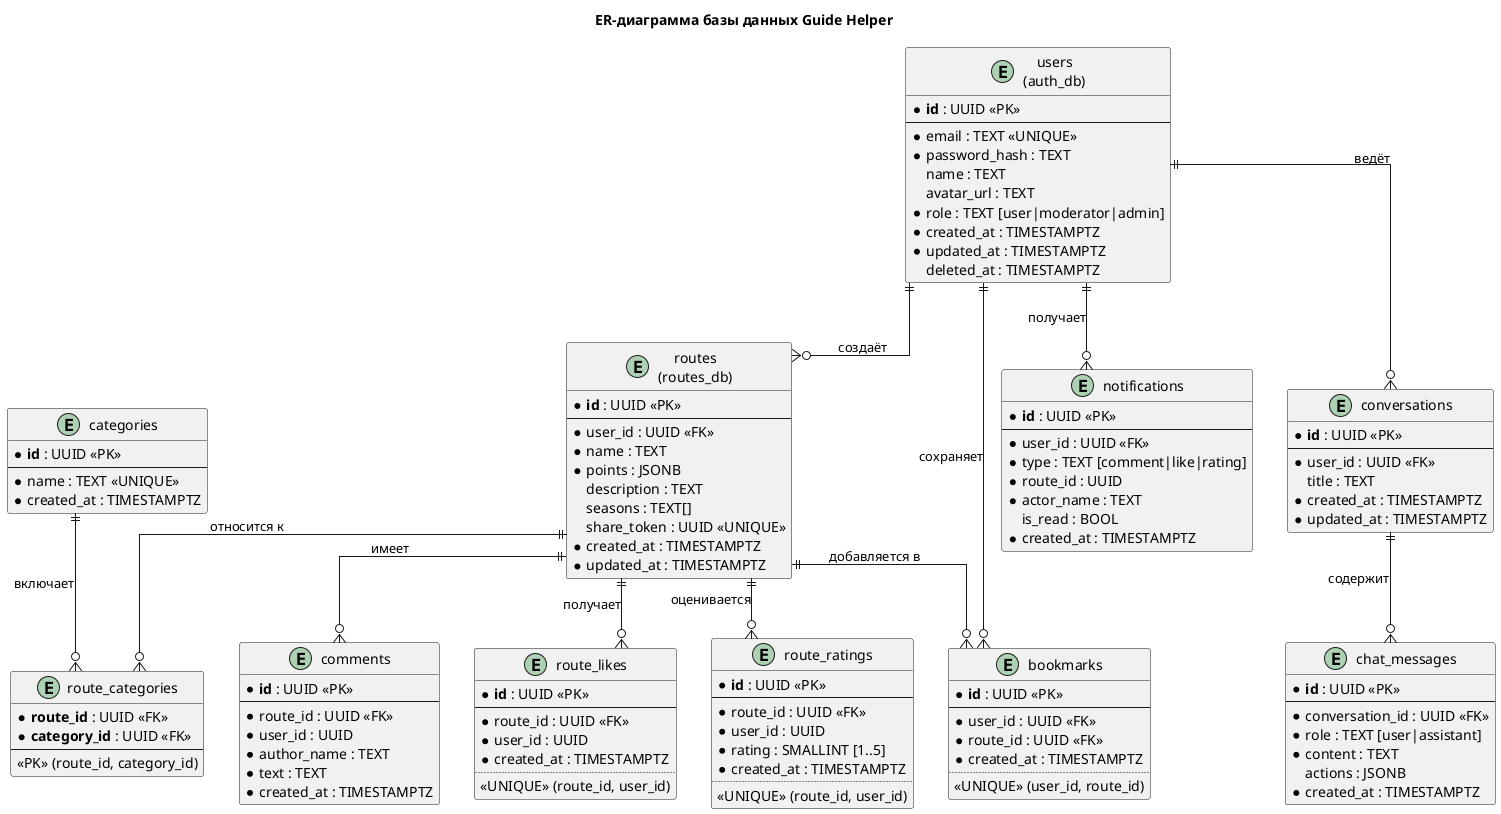
\includegraphics[width=0.85\textwidth]{images/er-diagram.png}
  \caption{ER-диаграмма базы данных}
  \label{fig:er-diagram}
\end{figure}


\section{Макеты страниц}
\label{sec:ui-mockups}

В данном разделе представлены макеты основных страниц работающего веб-приложения Guide Helper.

На рисунке~\ref{fig:mockup-map} представлена главная страница~--- редактор маршрутов с интерактивной картой. Пользователь может добавлять точки на карту, прикреплять к ним фотографии, строить маршрут между точками автоматически (через OSRM) или вручную. На правой панели отображаются статистики маршрута: расстояние, набор и сброс высоты, расчётное время в пути.

\begin{figure}[H]
  \centering
  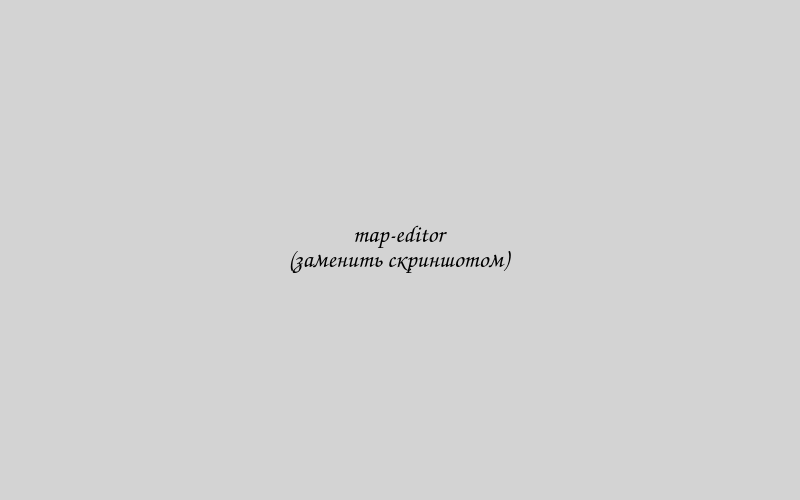
\includegraphics[width=0.95\textwidth]{images/mockups/map-editor.png}
  \caption{Редактор маршрутов с интерактивной картой}
  \label{fig:mockup-map}
\end{figure}

На рисунке~\ref{fig:mockup-shared} представлена страница публичного просмотра маршрута, доступная по уникальной ссылке. Отображается карта с маршрутом и фотографиями, комментарии, отметки «нравится» и рейтинг.

\begin{figure}[H]
  \centering
  
\includegraphics[width=0.95\textwidth]{images/mockups/shared-route.png}
  \caption{Страница публичного просмотра маршрута}
  \label{fig:mockup-shared}
\end{figure}

На рисунке~\ref{fig:mockup-profile} представлена страница профиля пользователя с вкладками: профиль, безопасность, список маршрутов. Пользователь может управлять своими маршрутами: просматривать, редактировать, удалять, экспортировать.

\begin{figure}[H]
  \centering
  
\includegraphics[width=0.95\textwidth]{images/mockups/profile.png}
  \caption{Страница профиля пользователя}
  \label{fig:mockup-profile}
\end{figure}

На рисунке~\ref{fig:mockup-explore} представлена страница каталога маршрутов. Пользователь может просматривать публичные маршруты других пользователей, фильтровать по категориям, сортировать по рейтингу, отметкам «нравится» и дате создания, а также выполнять текстовый поиск.

\begin{figure}[H]
  \centering
  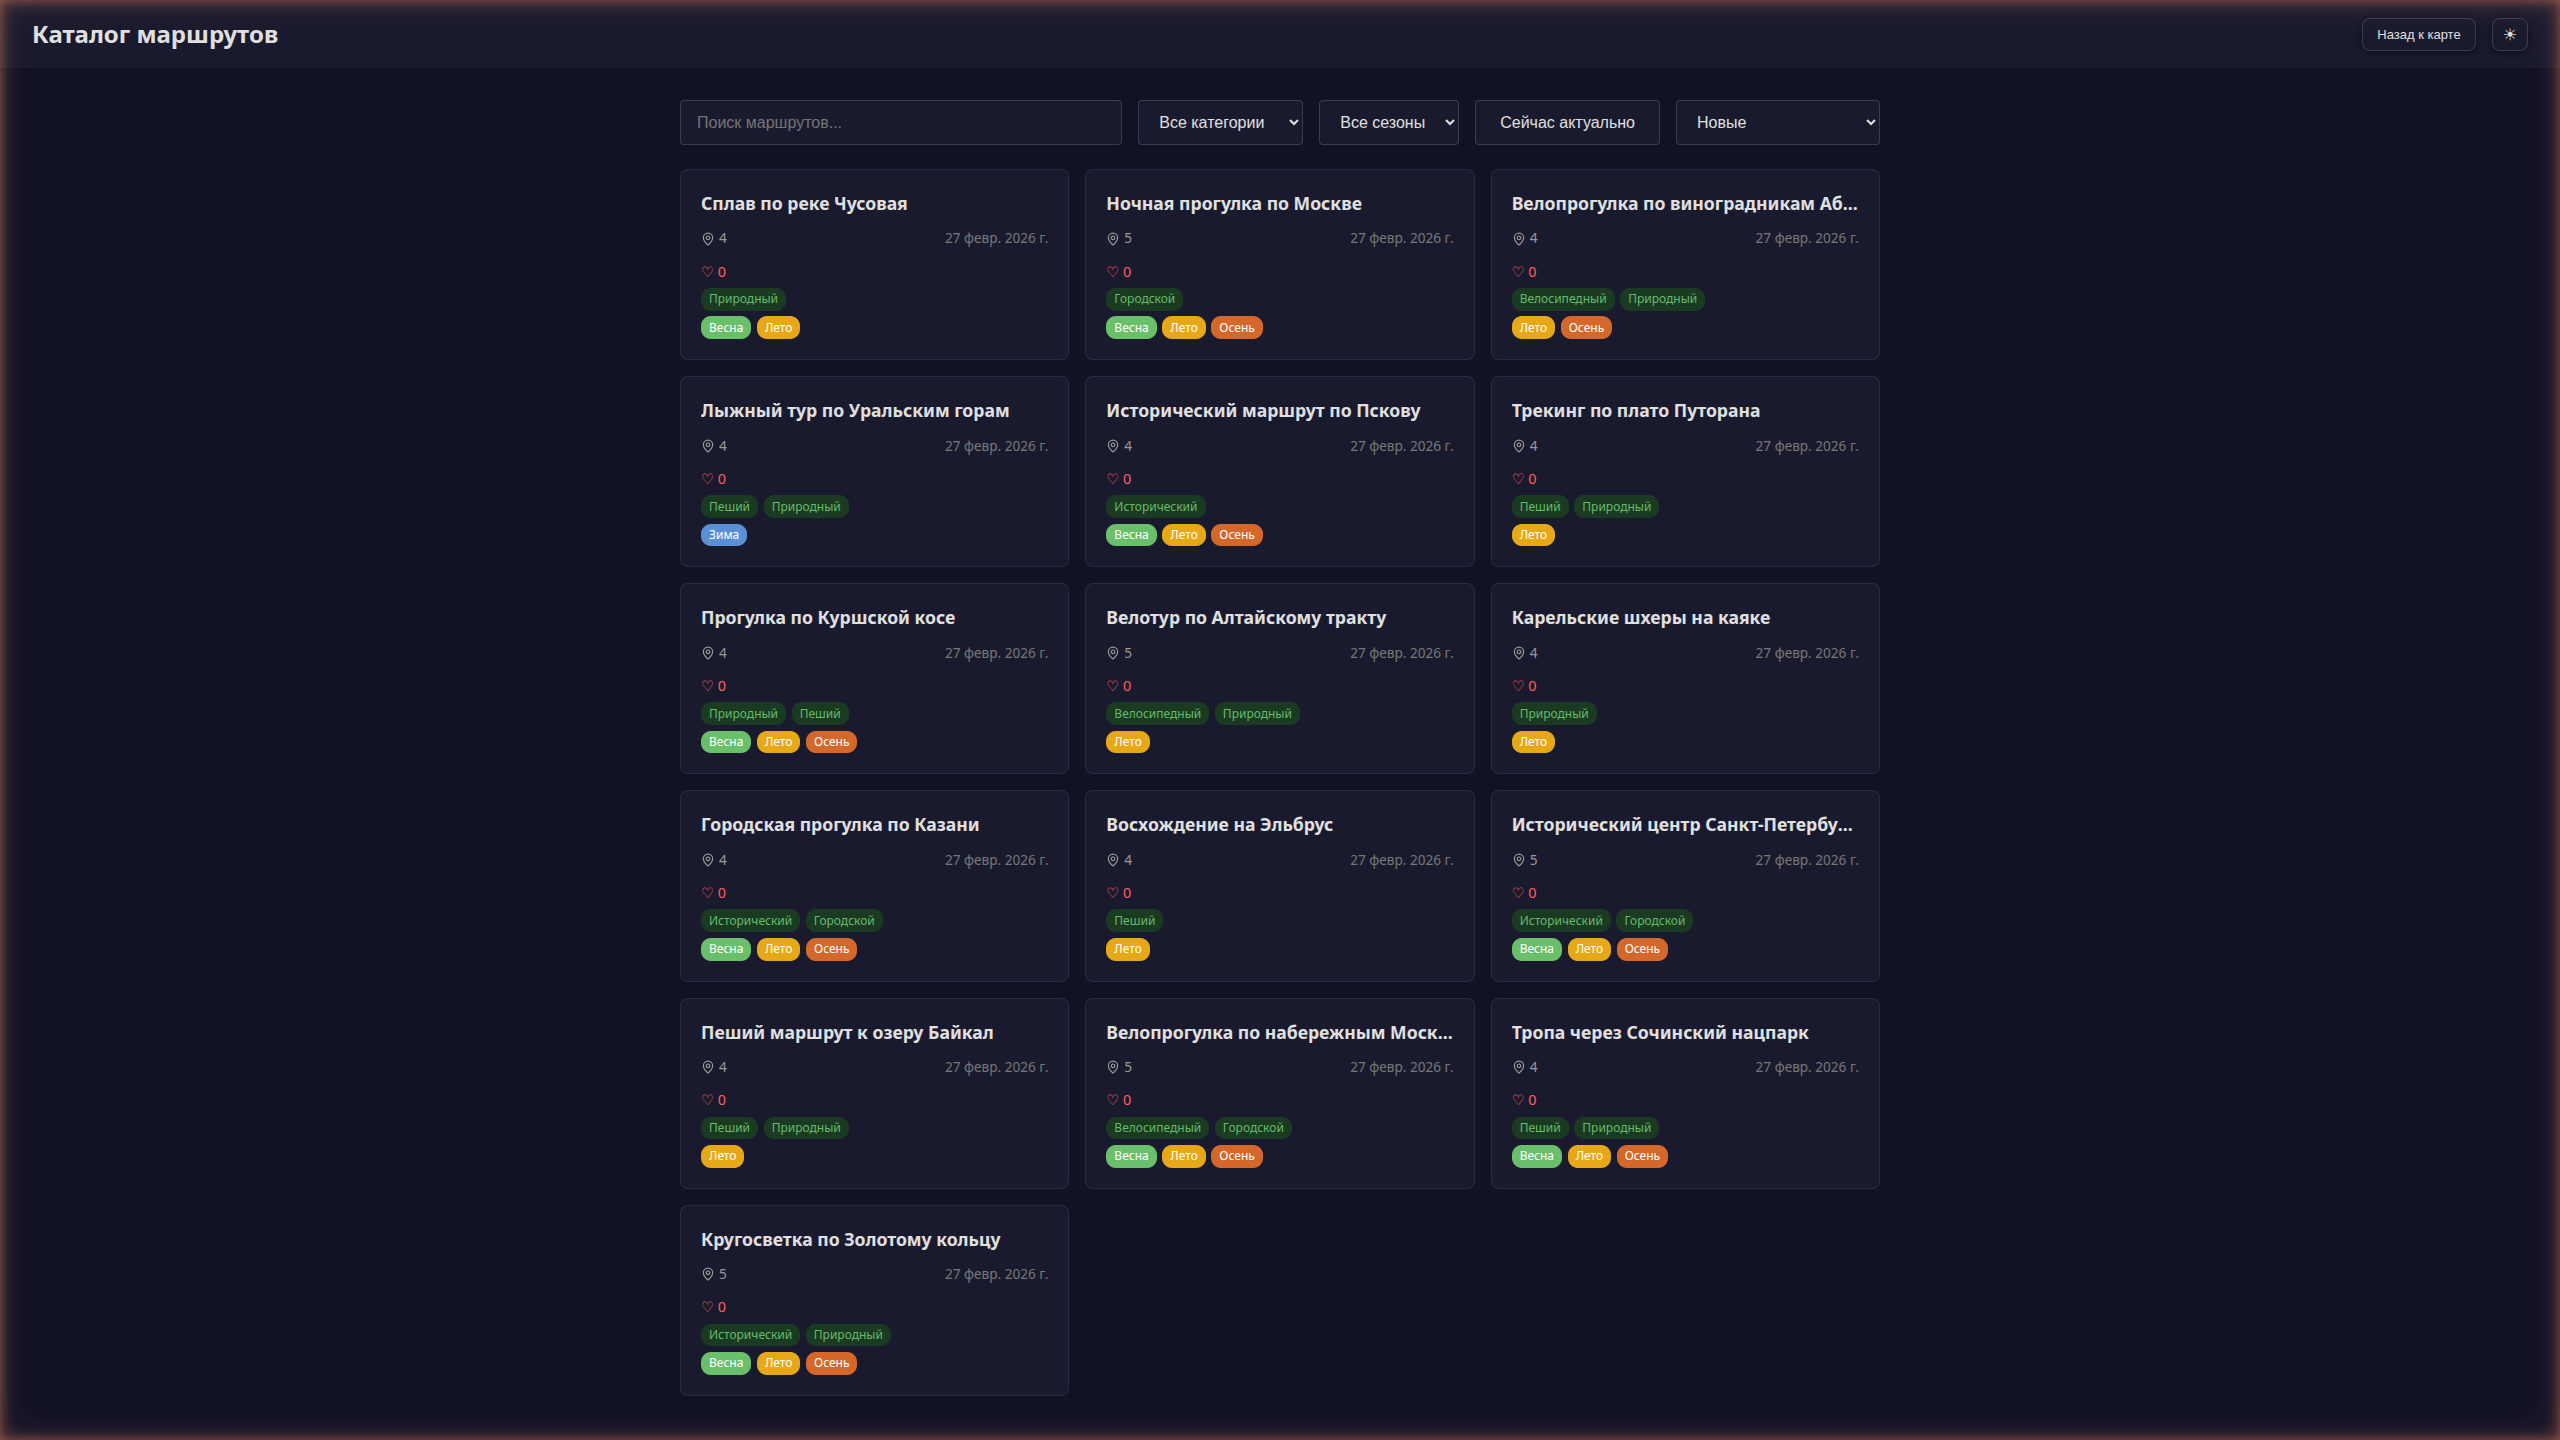
\includegraphics[width=0.95\textwidth]{images/mockups/explore.png}
  \caption{Каталог маршрутов}
  \label{fig:mockup-explore}
\end{figure}

Дополнительно в системе реализованы панель ИИ-ассистента (диалоговый интерфейс с вызовом инструментов для геокодирования, поиска маршрутов и навигации) и административная панель для управления пользователями, модерации контента и просмотра статистики системы.
